\begin{figure}[H]
    \centering
    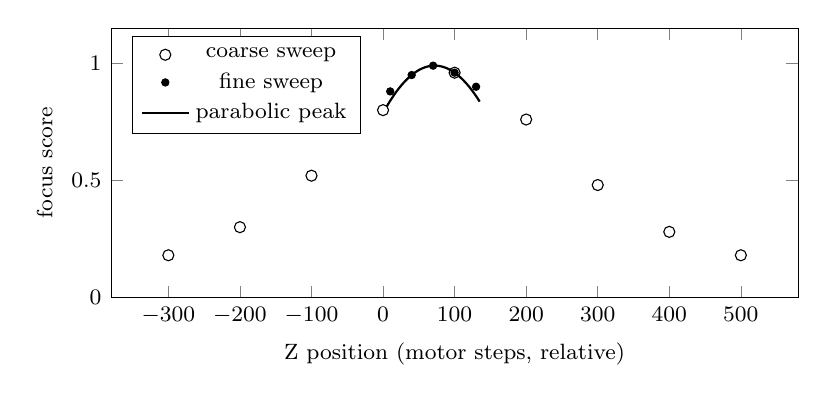
\begin{tikzpicture}
    \begin{axis}[width=0.85\linewidth, height=5cm,
        xlabel={Z position (motor steps, relative)}, ylabel={focus score},
        ymin=0, ymax=1.15, legend pos=north west,
        legend style={font=\footnotesize}, tick label style={font=\footnotesize},
        label style={font=\footnotesize}]
        \addplot[only marks, mark=o] coordinates {
            (-300,0.18)(-200,0.30)(-100,0.52)(0,0.80)(100,0.96)(200,0.76)(300,0.48)(400,0.28)(500,0.18)};
        \addplot[only marks, mark=*, mark size=1.3pt] coordinates {
            (10,0.88)(40,0.95)(70,0.99)(100,0.96)(130,0.90)};
        \addplot[domain=5:135, samples=60, thick] {-0.00003889*x*x + 0.005611*x + 0.7878};
        \legend{coarse sweep, fine sweep, parabolic peak}
    \end{axis}
    \end{tikzpicture}
    \caption[Two-stage autofocus sweep]{Schematic of the two-stage autofocus sweep. A coarse sweep brackets the approximate peak,
    a fine sweep refines around it, and a parabola fitted to the best fine sample and its two neighboring fine samples yields the sub-step focus position. The values shown are illustrative, not measured.}
    \label{fig:autofocus-sweep}
\end{figure}
